\newcommand{\adwareTagResultsAucTable}{
    \begin{table}[H]
        \centering
        \begin{tabular}{|p{2,8cm}||p{2,8cm} p{2,8cm} p{2,8cm}|}
            \hline
            Adware Tag & ALOHA & Joint Embedding & Proposed Model \\
            \hline
            AUC-ROC & \textBF{0.973$\pm$0.000} & 0.971$\pm$0.002 & 0.971$\pm$0.001 \\
            \hline
        \end{tabular}
        \caption{AUC-ROC (Area Under Curve) of the different models for the \textbf{Adware Tag} prediction task. Results were aggregated over \textBF{3} training runs with different weight initializations and minibatch orderings. Best results are shown in \textbf{bold}.} \label{tab:adwareTag_auc}
    \end{table}
}

\newcommand{\adwareTagResultsAtFprTable}{
    \begin{center}
        \begin{longtable}[c]{|p{3,2cm}||p{1,8cm} p{1,8cm} p{1,8cm} p{1,8cm} p{1,8cm}|}
            \hline
            Adware Tag & \multicolumn{5}{c|}{{FPR}} \\
            & $10^{-5}$ & $10^{-4}$ & $10^{-3}$ & $10^{-2}$ & $10^{-1}$ \\
            \hline
            \endfirsthead

            \caption*{\raggedright ...continued from previous page} \\
            \hline
            Adware Tag & \multicolumn{5}{c|}{\textbf{FPR}} \\
            & $10^{-5}$ & $10^{-4}$ & $10^{-3}$ & $10^{-2}$ & $10^{-1}$ \\
            \hline
            \endhead

            \caption*{\raggedleft ...continued on next page} \\
            \endfoot

            \caption{Mean and standard deviation results (TPR, Accuracy, Recall, Precision and F1-Score) of the different models for the \textbf{Adware Tag} prediction task at different \textbf{FPR}s (\textit{False Positive Rates}). Results were aggregated over \textBF{3} training runs with different weight initializations and minibatch orderings. Best results are shown in \textbf{bold}. Under \textbf{TPR} results are also presented the percentage reduction in mean detection error and in ROC curve standard deviation introduced by the \textit{Proposed Model} with respect to both \textit{ALOHA} model and \textit{Joint Embedding}.} \label{tab:adwareTag_results_at_fpr} \\
            \endlastfoot

            \multicolumn{6}{|c|}{\textbf{TPR}} \\
            \hline
            ALOHA & 0.129$\pm$0.017 & 0.256$\pm$0.029 & 0.453$\pm$0.047 & \textBF{0.719$\pm$0.006} & \textBF{0.934$\pm$0.010} \\
            Joint Embedding & \textBF{0.138$\pm$0.008} & \textBF{0.282$\pm$0.060} & \textBF{0.487$\pm$0.020} & 0.696$\pm$0.016 & 0.933$\pm$0.006 \\
            Proposed Model & 0.133$\pm$0.049 & 0.195$\pm$0.038 & 0.424$\pm$0.065 & 0.699$\pm$0.013 & 0.929$\pm$0.008 \\
            \hline
            Error Reduction wrt \newline ALOHA & 0.5\% & -8.2\% & -5.3\% & -7.1\% & -7.6\% \\
            Error Reduction wrt \newline Joint Embedding & -0.6\% & -12.1\% & -12.3\% & 1.0\% & -6.0\% \\
            \hline
            Std Reduction wrt \newline ALOHA & -188.2\% & -31.0\% & -38.3\% & -116.7\% & 20.0\% \\
            Std Reduction wrt \newline Joint Embedding & -512.5\% & 36.7\% & -225.0\% & 18.8\% & -33.3\% \\
            \hline
            \multicolumn{6}{|c|}{\textbf{Accuracy}} \\
            \hline
            ALOHA & 0.950$\pm$0.001 & 0.957$\pm$0.002 & 0.968$\pm$0.003 & \textBF{0.974$\pm$0.000} & 0.902$\pm$0.001 \\
            Joint Embedding & \textBF{0.950$\pm$0.000} & \textBF{0.959$\pm$0.003} & \textBF{0.970$\pm$0.001} & 0.973$\pm$0.001 & \textBF{0.902$\pm$0.000} \\
            Proposed Model & 0.950$\pm$0.003 & 0.954$\pm$0.002 & 0.966$\pm$0.004 & 0.973$\pm$0.001 & \textBF{0.902$\pm$0.000} \\
            \hline
            \multicolumn{6}{|c|}{\textbf{Recall}} \\
            \hline
            ALOHA & 0.129$\pm$0.017 & 0.256$\pm$0.029 & 0.453$\pm$0.047 & \textBF{0.719$\pm$0.006} & \textBF{0.934$\pm$0.010} \\
            Joint Embedding & \textBF{0.138$\pm$0.008} & \textBF{0.282$\pm$0.060} & \textBF{0.487$\pm$0.020} & 0.696$\pm$0.016 & 0.933$\pm$0.006 \\
            Proposed Model & 0.133$\pm$0.049 & 0.195$\pm$0.038 & 0.424$\pm$0.065 & 0.699$\pm$0.013 & 0.929$\pm$0.008 \\
            \hline
            \multicolumn{6}{|c|}{\textbf{Precision}} \\
            \hline
            ALOHA & \textBF{0.999$\pm$0.000} & \textBF{0.994$\pm$0.001} & 0.965$\pm$0.004 & \textBF{0.814$\pm$0.001} & 0.363$\pm$0.003 \\
            Joint Embedding & \textBF{0.999$\pm$0.000} & \textBF{0.994$\pm$0.001} & \textBF{0.967$\pm$0.001} & 0.809$\pm$0.003 & \textBF{0.363$\pm$0.002} \\
            Proposed Model & 0.999$\pm$0.001 & 0.991$\pm$0.001 & 0.962$\pm$0.005 & 0.810$\pm$0.003 & 0.362$\pm$0.002 \\
            \hline
            \multicolumn{6}{|c|}{\textbf{F1 Score}} \\
            \hline
            ALOHA & 0.228$\pm$0.027 & 0.406$\pm$0.037 & 0.615$\pm$0.045 & \textBF{0.764$\pm$0.004} & 0.523$\pm$0.004 \\
            Joint Embedding & \textBF{0.243$\pm$0.012} & \textBF{0.436$\pm$0.074} & \textBF{0.647$\pm$0.018} & 0.748$\pm$0.010 & \textBF{0.523$\pm$0.003} \\
            Proposed Model & 0.231$\pm$0.077 & 0.324$\pm$0.052 & 0.586$\pm$0.063 & 0.750$\pm$0.009 & 0.521$\pm$0.003 \\
            \hline
        \end{longtable}
    \end{center}
}

\newcommand{\adwareTagResultsSummaryTable}{
    \begin{table}[H]
        \centering
        \begin{tabular}{|p{3,2cm}||p{1,8cm} p{1,8cm} p{1,8cm} p{1,8cm} p{1,8cm}|}
            \hline
            \multicolumn{6}{|c|}{Adware Tag (at FPR $=1\%$)} \\
            \hline
            Model & TPR & Accuracy & Precision & Recall & F1 score \\
            \hline
            ALOHA & \textBF{0.719$\pm$0.006} & \textBF{0.974$\pm$0.000} & \textBF{0.814$\pm$0.001} & \textBF{0.719$\pm$0.006} & \textBF{0.764$\pm$0.004} \\
            Joint Embedding & 0.696$\pm$0.016 & 0.973$\pm$0.001 & 0.809$\pm$0.003 & 0.696$\pm$0.016 & 0.748$\pm$0.010 \\
            Proposed Model & 0.699$\pm$0.013 & 0.973$\pm$0.001 & 0.810$\pm$0.003 & 0.699$\pm$0.013 & 0.750$\pm$0.009 \\
            \hline
        \end{tabular}
        \caption{Summary of the mean and standard deviation results of the different models for the \textbf{Adware Tag} prediction task at \textbf{FPR} $=1\%$. Results were aggregated over \textBF{3} training runs with different weight initializations and minibatch orderings. Best results are shown in \textbf{bold}.} \label{tab:adwareTag_result_summary}
    \end{table}
}

\newcommand{\adwareTagRocAloha}{
    \begin{figure}[H]
        \vspace*{-0.5cm}
        \centering
        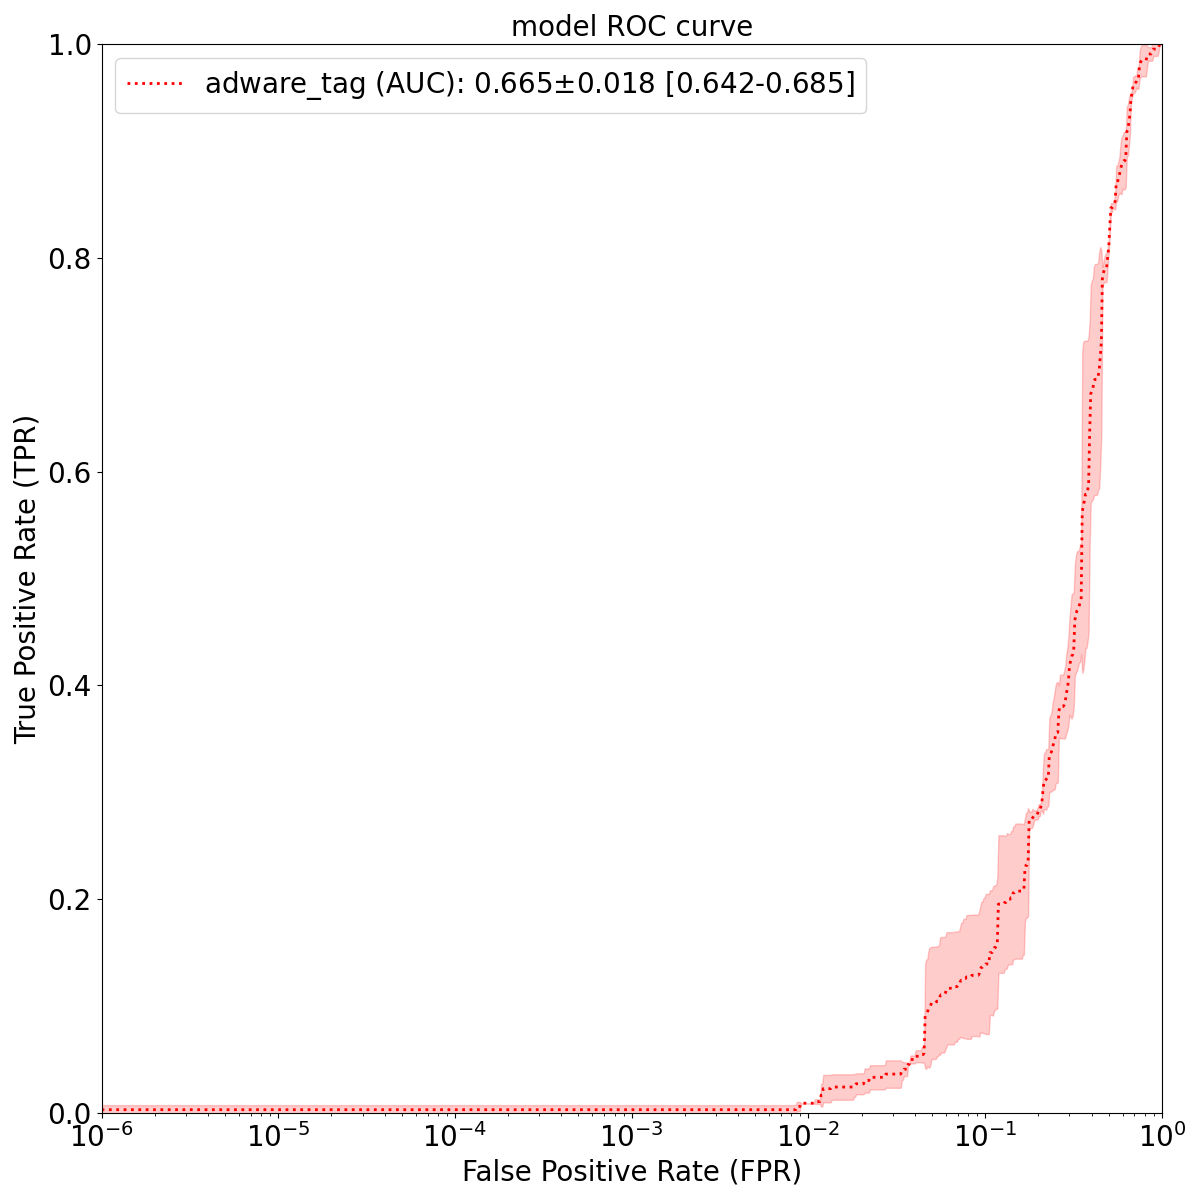
\includegraphics[width=0.6\textwidth]{./results/adware_tag_roc_aloha.png}
        \vspace*{-0.2cm}
        \caption{ROC curve and AUC statistics of \textBF{ALOHA} model for the \textbf{Adware Tag}. The line represents the \textit{mean} TPR at a given FPR, while the shaded region represents the \textit{standard deviation}. Statistics were computed over \textBF{3} training runs, each with random parameter initialization.}
        \label{fig:adwareTagRocAloha}
    \end{figure}
}

\newcommand{\adwareTagRocJointEmbedding}{
    \begin{figure}[H]
        \vspace*{-0.5cm}
        \centering
        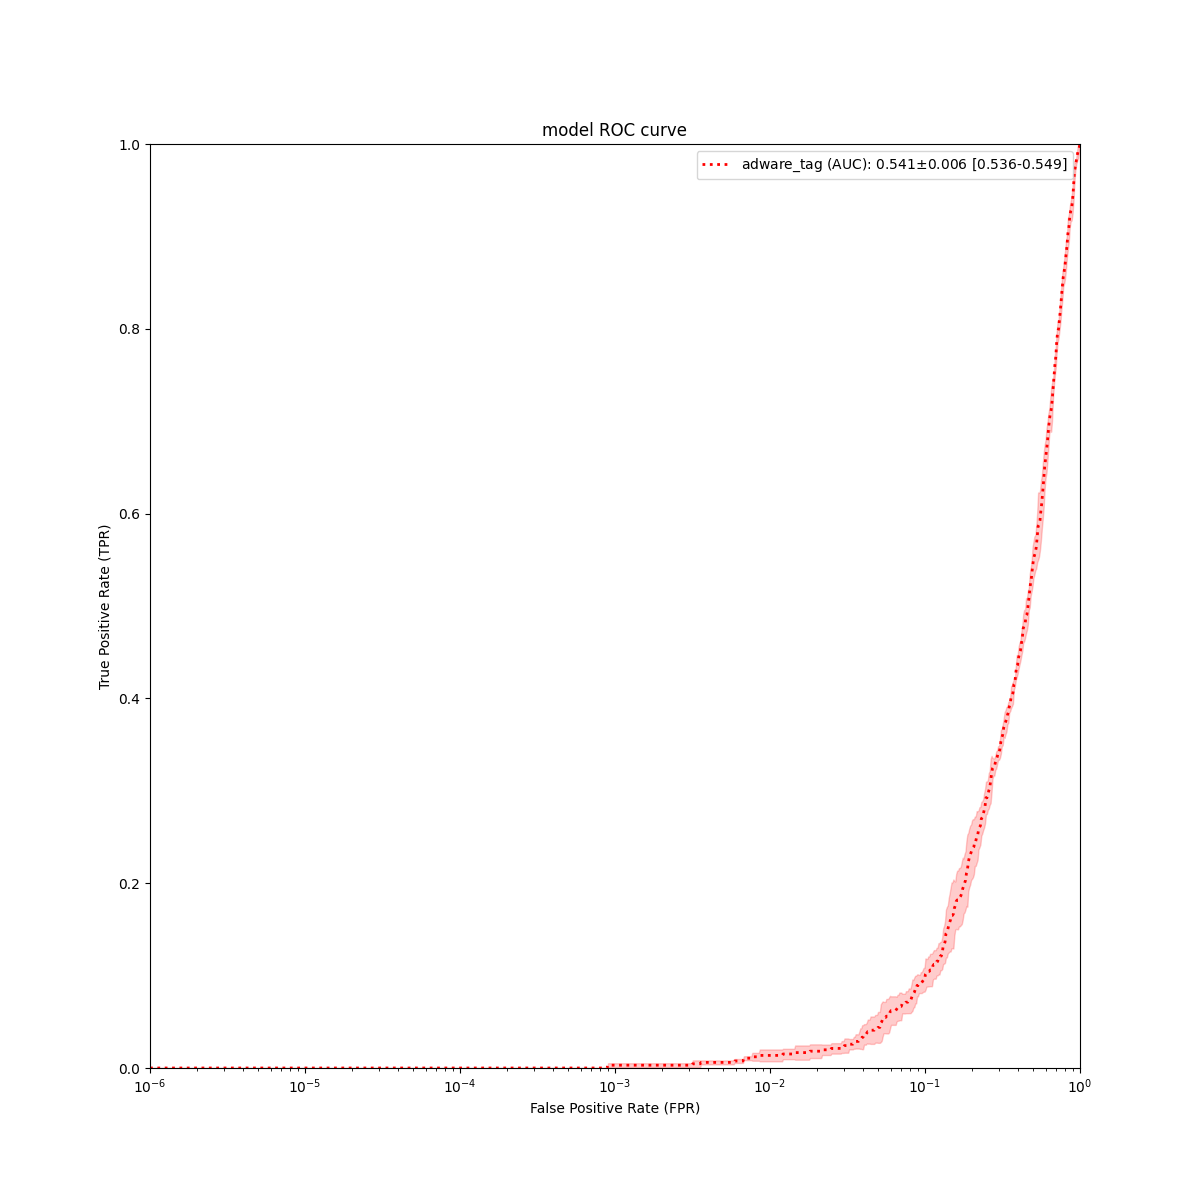
\includegraphics[width=0.6\textwidth]{./results/adware_tag_roc_jointEmbedding.png}
        \vspace*{-0.2cm}
        \caption{ROC curve and AUC statistics of \textBF{Joint Embedding} model for the \textbf{Adware Tag}. The line represents the \textit{mean} TPR at a given FPR, while the shaded region represents the \textit{standard deviation}. Statistics were computed over \textBF{3} training runs, each with random parameter initialization.}
        \label{fig:adwareTagRocJointEmbedding}
    \end{figure}
}

\newcommand{\adwareTagRocProposedMethod}{
    \begin{figure}[H]
        \vspace*{-0.5cm}
        \centering
        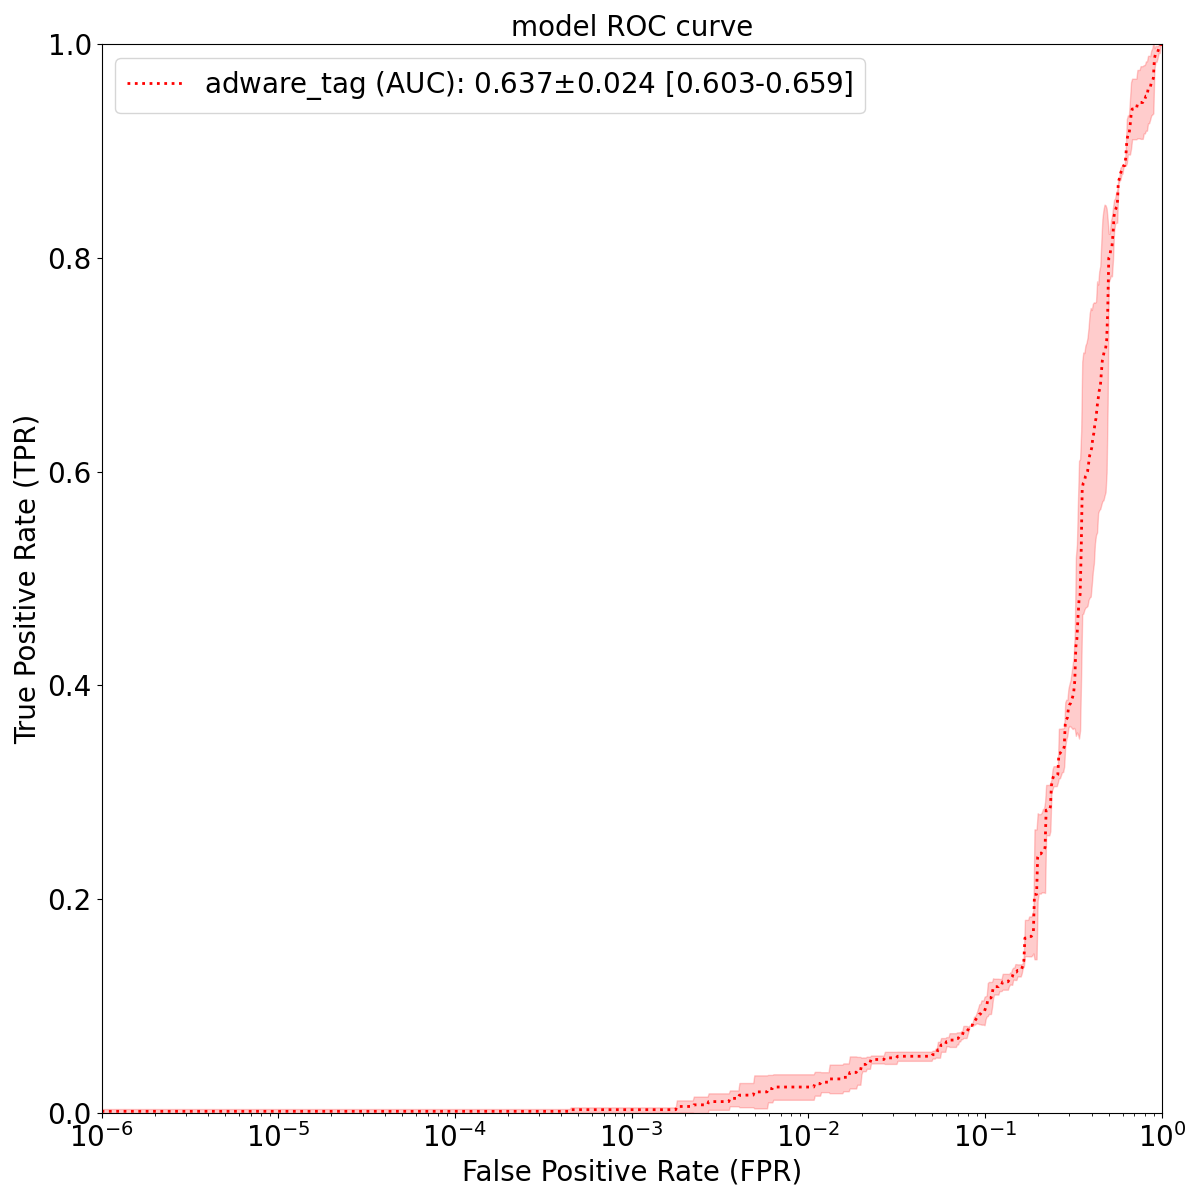
\includegraphics[width=0.6\textwidth]{./results/adware_tag_roc_proposedModel.png}
        \vspace*{-0.2cm}
        \caption{ROC curve and AUC statistics of \textBF{Proposed Model} for the \textbf{Adware Tag}. The line represents the \textit{mean} TPR at a given FPR, while the shaded region represents the \textit{standard deviation}. Statistics were computed over \textBF{3} training runs, each with random parameter initialization.}
        \label{fig:adwareTagRocProposedModel}
    \end{figure}
}
